\documentclass[normal,cyan]{elegantnote}
\usepackage{float}
\usepackage{diagbox}

\title{信息论复习资料\footnotemark[1]}
\author{CharlesLC\footnotemark[2]}
\institute{建模小组成员}
\version{1.00}
\date{\zhtoday}
\newcommand{\nl}{\underline{\makebox[2em]{}}}
\begin{document}
\maketitle
\section*{\centering \zihao{1}声明}
\hspace*{1cm} {\heiti\zihao{1}本页非正文!!!}   {\heiti\zihao{1}本页非正文!!!} \par
{\heiti\zihao{3}该文档是学长发的资料整理的,不保证答案的}{\heiti\zihao{2}正确性},{\heiti\zihao{3}使用者在考试时所有的损害},{\heiti\zihao{2}本人不承担任何伤害。}\par
{\heiti\zihao{3}该文档是学长发的资料整理的,不保证答案的}{\heiti\zihao{2}正确性},{\heiti\zihao{3}使用者在考试时所有的损害},{\heiti\zihao{2}本人不承担任何伤害。}\par 
{\heiti\zihao{3}该文档是学长发的资料整理的,不保证答案的}{\heiti\zihao{2}正确性},{\heiti\zihao{3}使用者在考试时所有的损害},{\heiti\zihao{2}本人不承担任何伤害。}\par 
{\heiti\zihao{3}正文内容从}{\heiti\zihao{2}第二页}\ \ {\heiti\zihao{3}开始。}{\heiti\zihao{3}正文内容从}{\heiti\zihao{2}第二页}{\heiti\zihao{3}开始。}\par
{\heiti\zihao{2}如需复制,请从第二页开始复制!!!}\par
\vspace*{1cm}
{\heiti\zihao{1}未}{\heiti\zihao{2}经}{\heiti\zihao{1}本}{\heiti\zihao{2}人}
{\heiti\zihao{1}允}{\heiti\zihao{2}许,}{\heiti\zihao{1}不}{\heiti\zihao{2}得}{\heiti\zihao{1}随}{\heiti\zihao{2}意}{\heiti\zihao{1}传}
{\heiti\zihao{2}播。}\par
{\heiti\zihao{1}未}{\heiti\zihao{2}经}{\heiti\zihao{1}本}{\heiti\zihao{2}人}
{\heiti\zihao{1}允}{\heiti\zihao{2}许,}{\heiti\zihao{1}不}{\heiti\zihao{2}得}{\heiti\zihao{1}随}{\heiti\zihao{2}意}{\heiti\zihao{1}传}
{\heiti\zihao{2}播。}

\footnotetext[1]{仅供学习使用,禁止商业用途}
\footnotetext[2]{\href{https://github.com/1411279054}{CharlesLC}制作}
\footnotetext[3]{感谢\href{https://github.com/pylittlebrat}{pylittlebrat}提供资源}
\footnotetext[4]{推荐大佬\href{https://github.com/jiangjk2000}{jiangjk2000}可咨询网络、服务器问题}
\thispagestyle{empty}
\newpage
\section*{\centering  \zihao{2}{信息论基础复习课}}
\section*{基本概念、性质和定理}
\begin{enumerate}
    \item 必然事件的自信息量是\nl,对于任一事件~$X_k$, 其自信息的值越大,说明事件
    $X_k$\nl。
    \item 当随机变量相互独立时,条件熵$H(X|Y)$与信源熵$H(X)$的关系是\nl。
    \item 对于离散无记忆信源,当信源熵有最大值时,满足条件为\nl。
    \item 对于连续信源来说,当输出幅度受限时,服从\nl 分布的随机变量具有最大熵; 
    \item 对于平均功率受限的连续随机变量,服从\nl 分布时具有最大熵。
    \item 按信源发出符号所对应得随机变量之间有无统计依赖关系,可将离散信源分为\nl 和\nl 两大类。
    \item 当\nl 时,信源与信道达到匹配。
    \item 信源编码得主要目的是\nl,信道编码的主要目的\nl。
    \item 费诺编码比较合适于\nl 的信源。
    \item 设有一离散无记忆平稳信道,其信道容量为$C$,只有待传送的信息传输率$R$与信道容量$C$满足\nl,则存在一种编码,当输入序列长度$n$足够答,使译码错误率任意小。
    \item 非奇异码是指一种分租码中的所有码字都\nl 的码。
    \item 费诺编码比较合适于\nl 的信源。
\end{enumerate}
\section*{信息量的计算}
\subsection*{一、自信息、条件自信息等的计算}
\begin{enumerate}
    \item 一个布袋内放~100~个球,其中~80~个球为红色,20~个球为白色。若随机摸取一个球,猜测其颜色,求平均摸取一次所获得的信息量。
    \vspace*{0.8cm}
    \item 一副充分洗乱了的牌(52张),问
    \begin{enumerate}
        \item   任一特定排列所给出的信息量是多少?
        \item   从中抽出13张牌,所给出的点数都不相同时得到多少信息量?
    \end{enumerate}
    \vspace*{0.8cm}
    \item 一个汽车牌照编号系统使用3个字母后接3个数字作代码,问一个牌照所提供的信息量是多少?如果所有6个字符都用字母数字做代码,问一个拍照所提供的信息量是多少?(假定有26个字母,10个数字。)
    \vspace*{0.8cm}
    \item 某地区的女孩中有20\%是大学生,在女大学生中有80\%是身高1.6米以上的,而女孩中身高1.6米以上的占总数的一半。假如我们得知“身高1.6米以上的某女孩是大学”的消息,问获得多少信息量?
\end{enumerate}
\subsection*{二、离散型随机变量的熵、平均互信息、联合熵、噪声熵、损失熵(信道疑义度)、条件熵}
\begin{enumerate}
    \item 随机掷三颗骰子,以$X$表示第一颗骰子抛掷的结果,以$Y$表示第一颗和第二颗骰子抛掷之和,以$Z$表示三颗骰子的点数之和,试求$H(X|Y)$,$H(Z|X,Y)$和$H(X,Z|Y)$。
    \vspace*{0.8cm}
    \item 把已知信源
    $
    \begin{bmatrix}
        X\\P
    \end{bmatrix}
    $  = $\begin{bmatrix}
        x_1 & x_2\\
        0.5 & 0.5 
    \end{bmatrix}$,接到如下图所示的信道上,
    \begin{figure}[H]
        \centering
        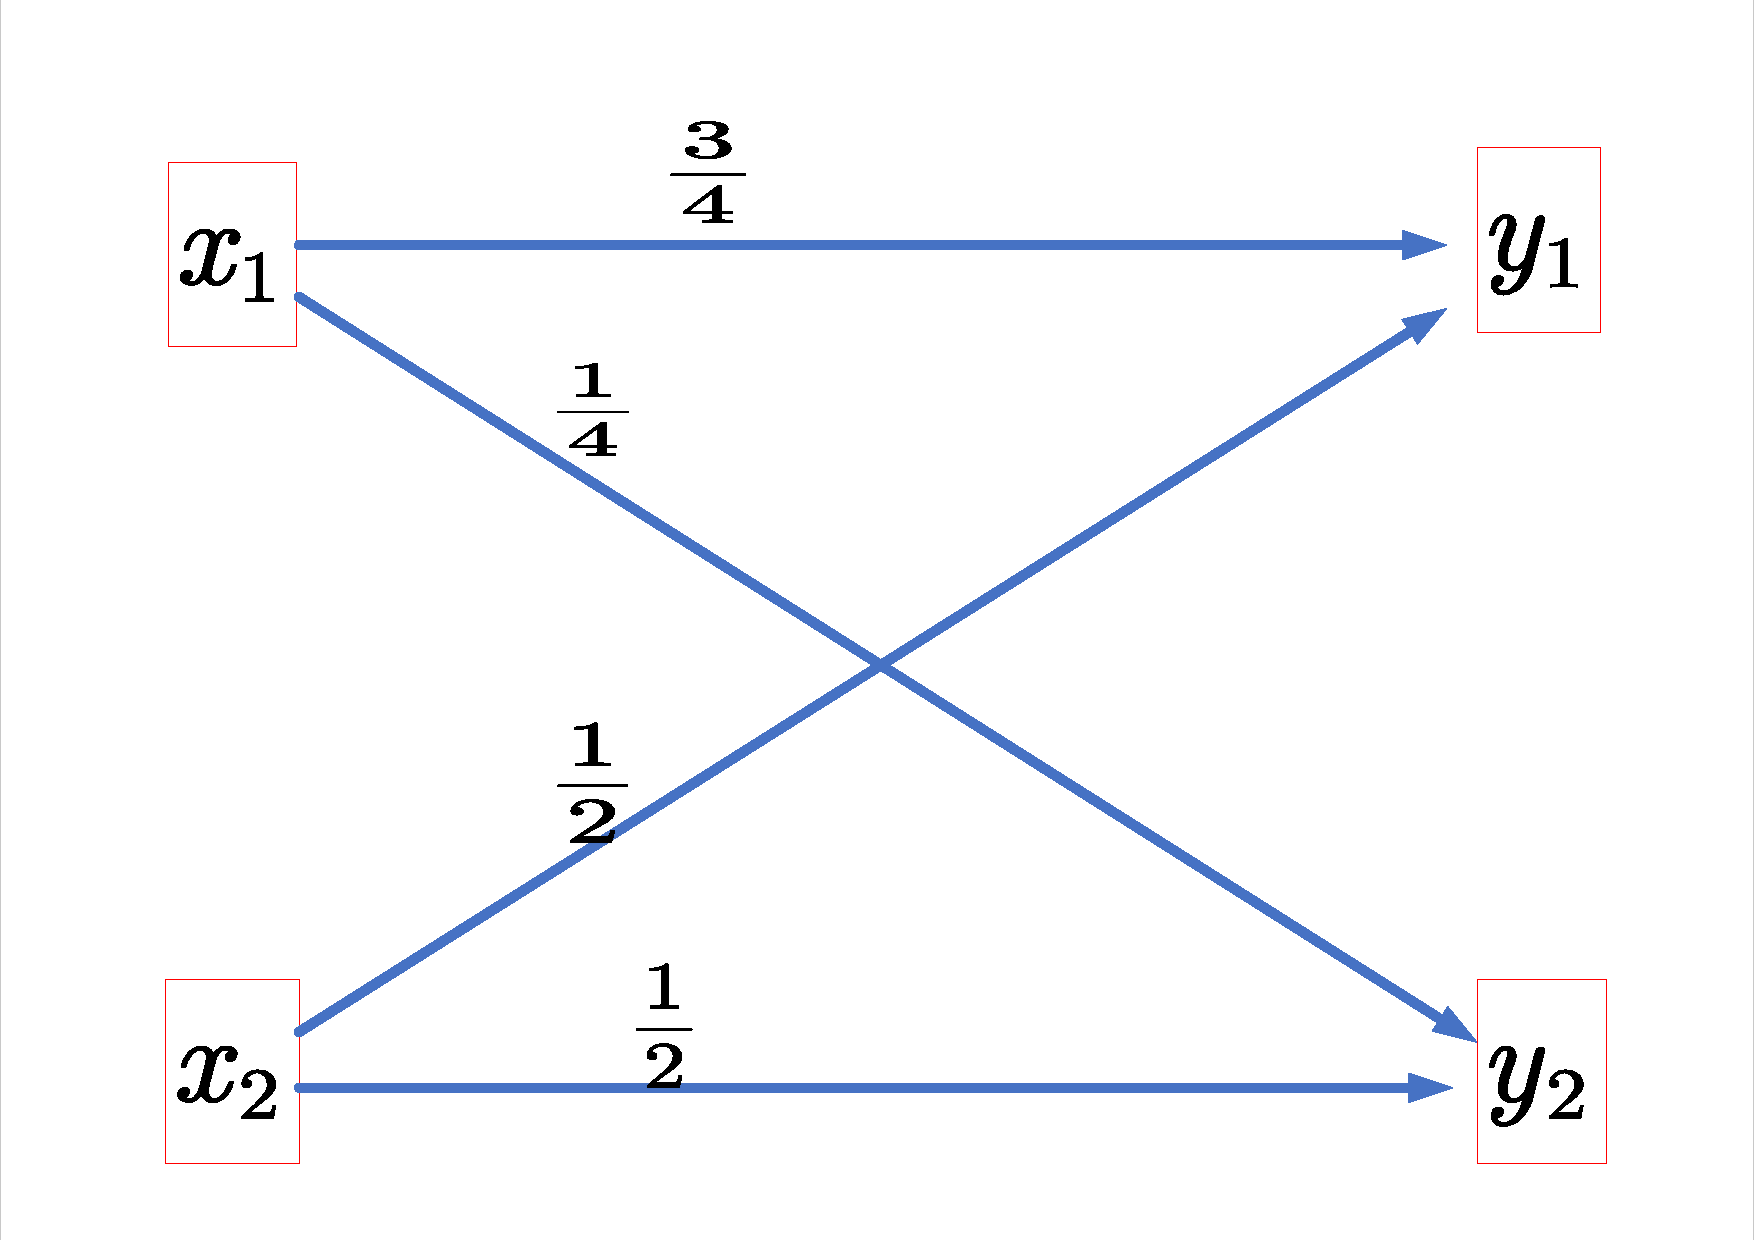
\includegraphics[width=0.45\textwidth]{figure/fig1.pdf}
    \end{figure}
    求在该信道上传输的平均互信息量$I(X;Y)$、噪声熵$H(Y|X)$和联合熵$H(X,Y)$。
    \vspace*{0.8cm}
    \item 把已知信源$\begin{bmatrix}
        X\\
        P
    \end{bmatrix}$=$\begin{bmatrix}
        x_1 & x_2\\
        0.5 & 0.5 \\
    \end{bmatrix}$接到如下图所示的信道上,
    \begin{figure}[H]
        \centering
        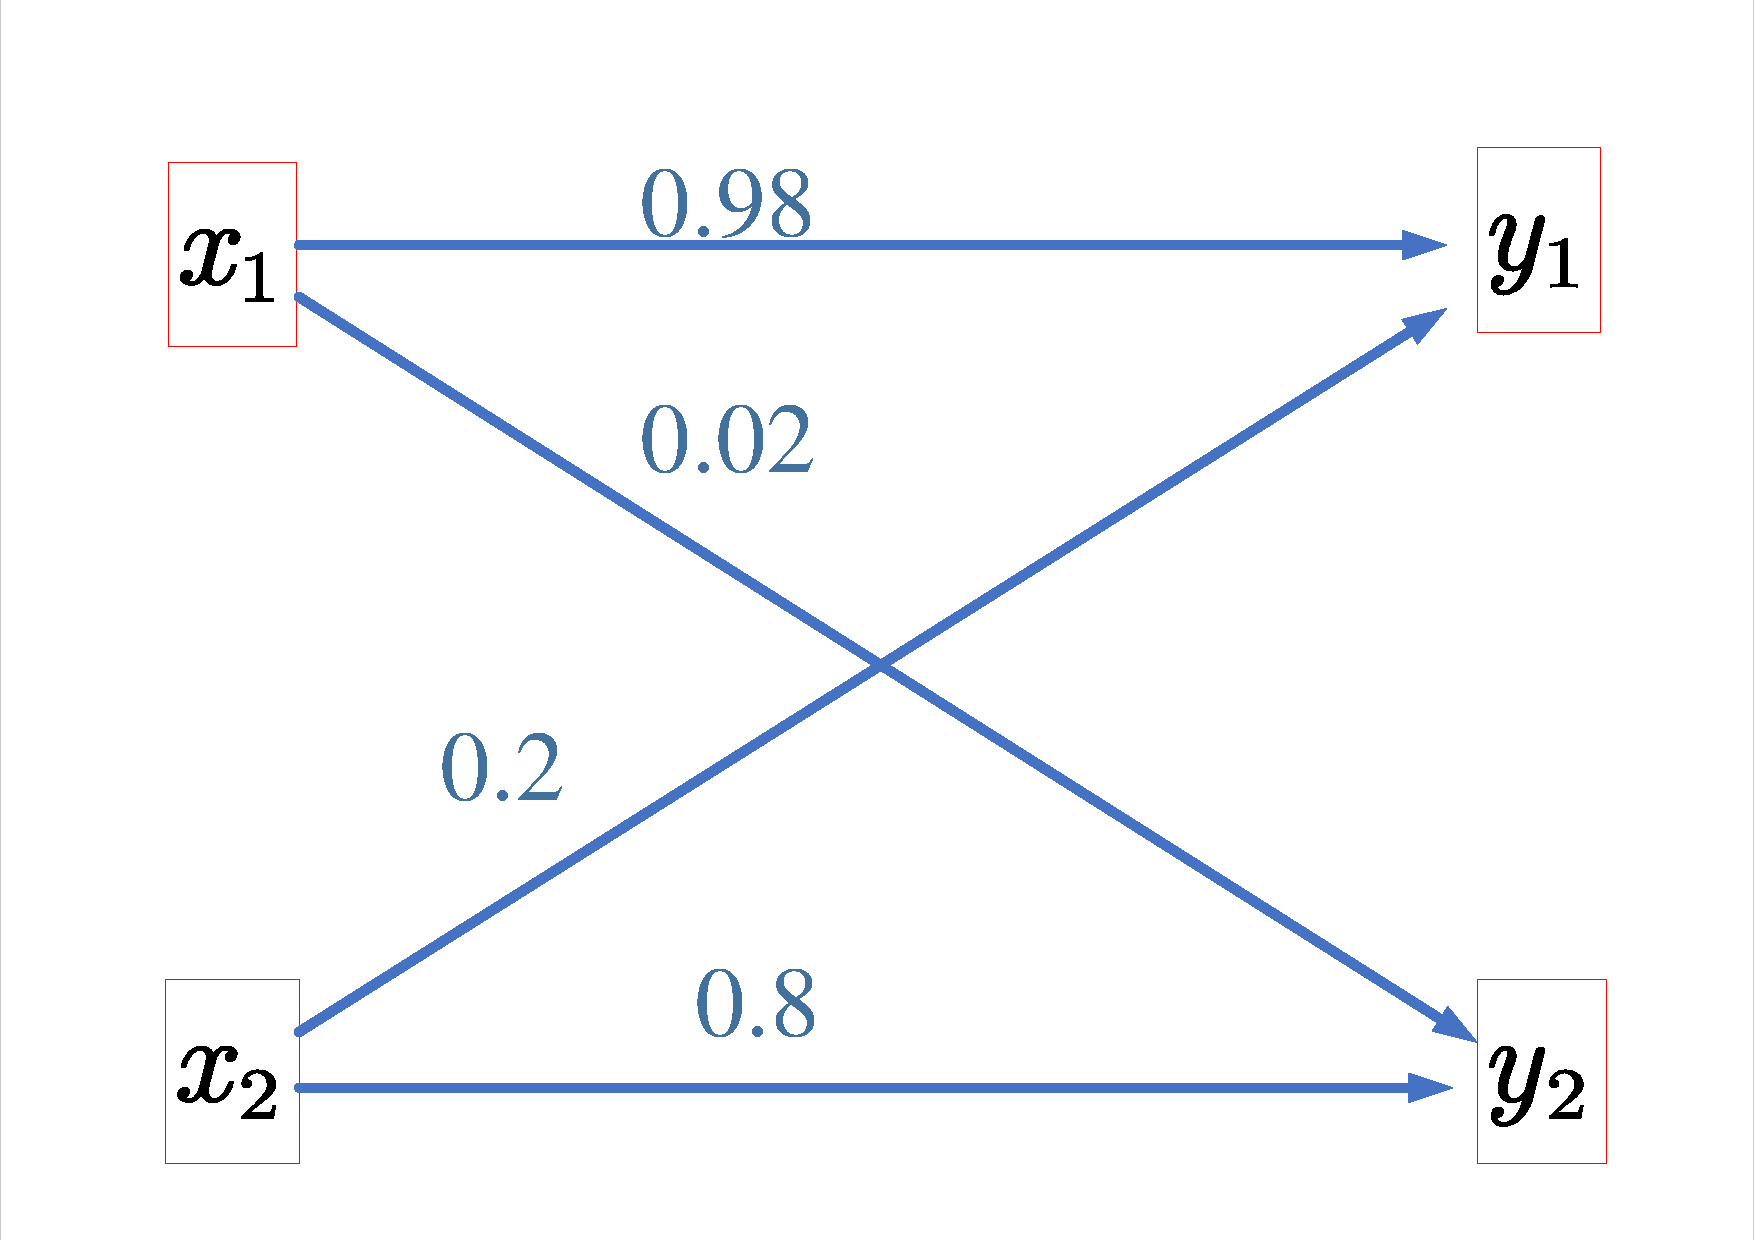
\includegraphics[width=0.45\textwidth]{figure/fig2.pdf}
    \end{figure}
    求在该信道上传输的平均互信息量$I(X;Y)$、噪声熵$H(Y|X)$和联合熵$H(X,Y)$。
    \vspace*{0.8cm}
    \item 有两个二元随机变量$X$和$Y$,它们的联合概率为
    \begin{table}[H]
        \centering
        \begin{tabular}{|c|c|c|}
            \hline
            \diagbox{$Y$}{$X$} & $x_1=0$ & $x_2=1$ \\
            \hline
            $y_1=0$ & $\frac{1}{8}$ & $\frac{3}{8}$ \\[6pt]
            \hline
            $y_2=1$ & $\frac{3}{8}$ & $\frac{1}{8}$\\[6pt]
            \hline
        \end{tabular}
    \end{table}
    并定义另一随机变量$Z=XY$(一般乘积),试计算:$I(Y;Z|X)$和$I(X;Z|Y)$。
\end{enumerate}
\subsection*{三、连续型随机变量及随机变量函数的熵}
\begin{enumerate}
    \item  设$X$是[-1,1]上的均匀分布随机变量,试求$H_C(X)$,$H_C(X^2)$。
    \vspace*{0.8cm}
    \item  设一个连续随机变量的概率密度为:$p(x)=\begin{cases}
        A\mathrm{cos}x & |x|\le \frac{\pi}{2}\\
        0 & \text{其他}
    \end{cases}$,又有$\displaystyle{\int_{-\pi/2}^{\pi/2}p(x)=1}$,求此随机变量的熵。
\end{enumerate}
\subsection*{四、马尔科夫信源:状态转移概率矩阵、状态转移图、过渡状态、遍历状态、状态平稳分布、极限熵(符号熵)}
\begin{enumerate}
    \item 一马氏链如图所示:
    \begin{figure}[H]
        \centering
        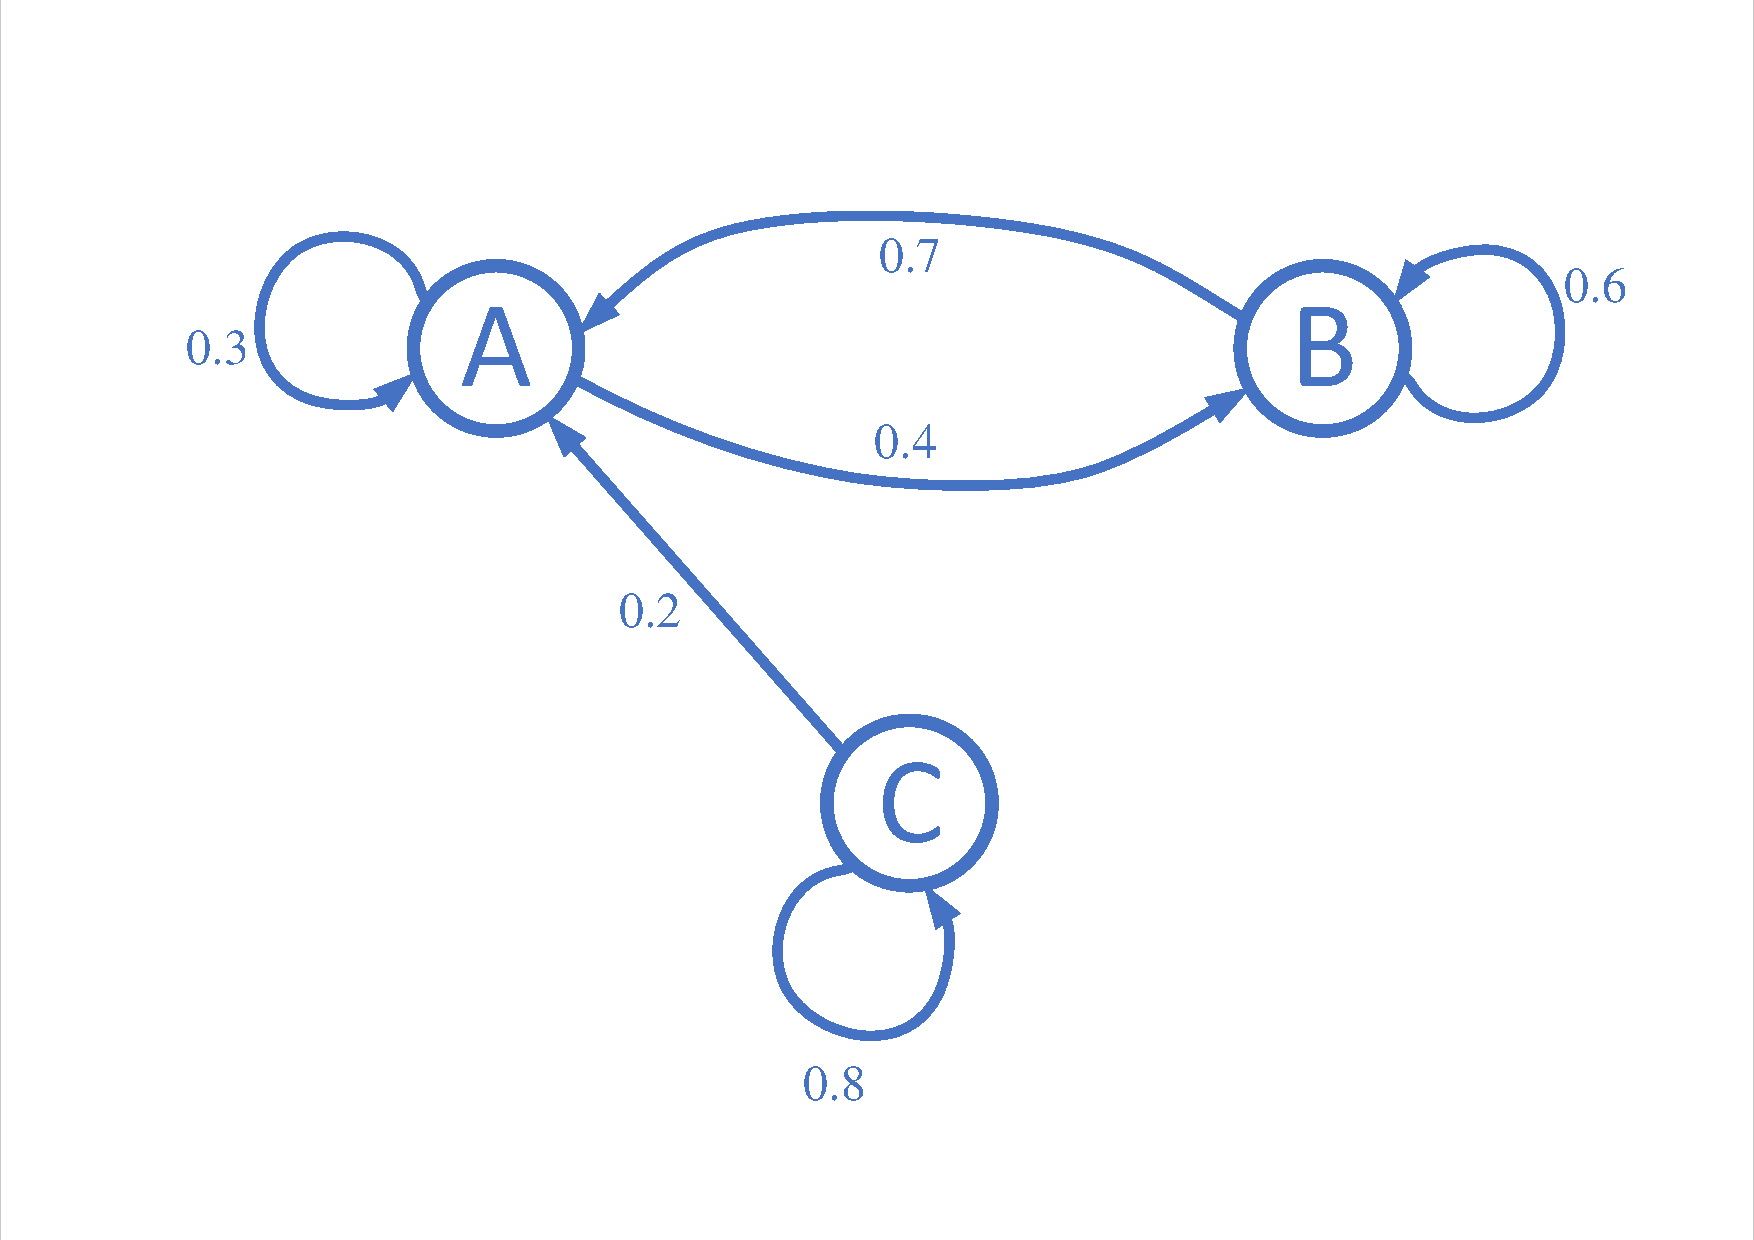
\includegraphics[width=0.45\textwidth]{figure/fig3.pdf}
    \end{figure}
    \begin{enumerate}
        \item 写出状态转移概率矩阵;
        \vspace*{0.3cm}
        \item 确定过渡状态和遍历状态;
        \vspace*{0.3cm}
        \item 求状态平稳分布。
    \end{enumerate}
    \vspace*{0.8cm}
    \item 一个三状态马尔科夫信源的转移概率矩阵
    P=$\begin{bmatrix}
        1/2 & 0 & 1/2 \\
        1/2 & 1/2 & 0 \\
        1/4 & 1/2 & 1/4 \\
    \end{bmatrix}$
    \begin{enumerate}
        \item  绘制状态转移图;
        \vspace*{0.3cm}
        \item 求该马尔科夫信源的稳态分布;
        \vspace*{0.3cm}
        \item 求极限熵;
    \end{enumerate}
    \vspace*{0.8cm}
    \item 一个一阶马氏源的状态转移图如下图所示,信源的符号集为$\left\{0,1,2\right\}$
    \begin{figure}[H]
        \centering
        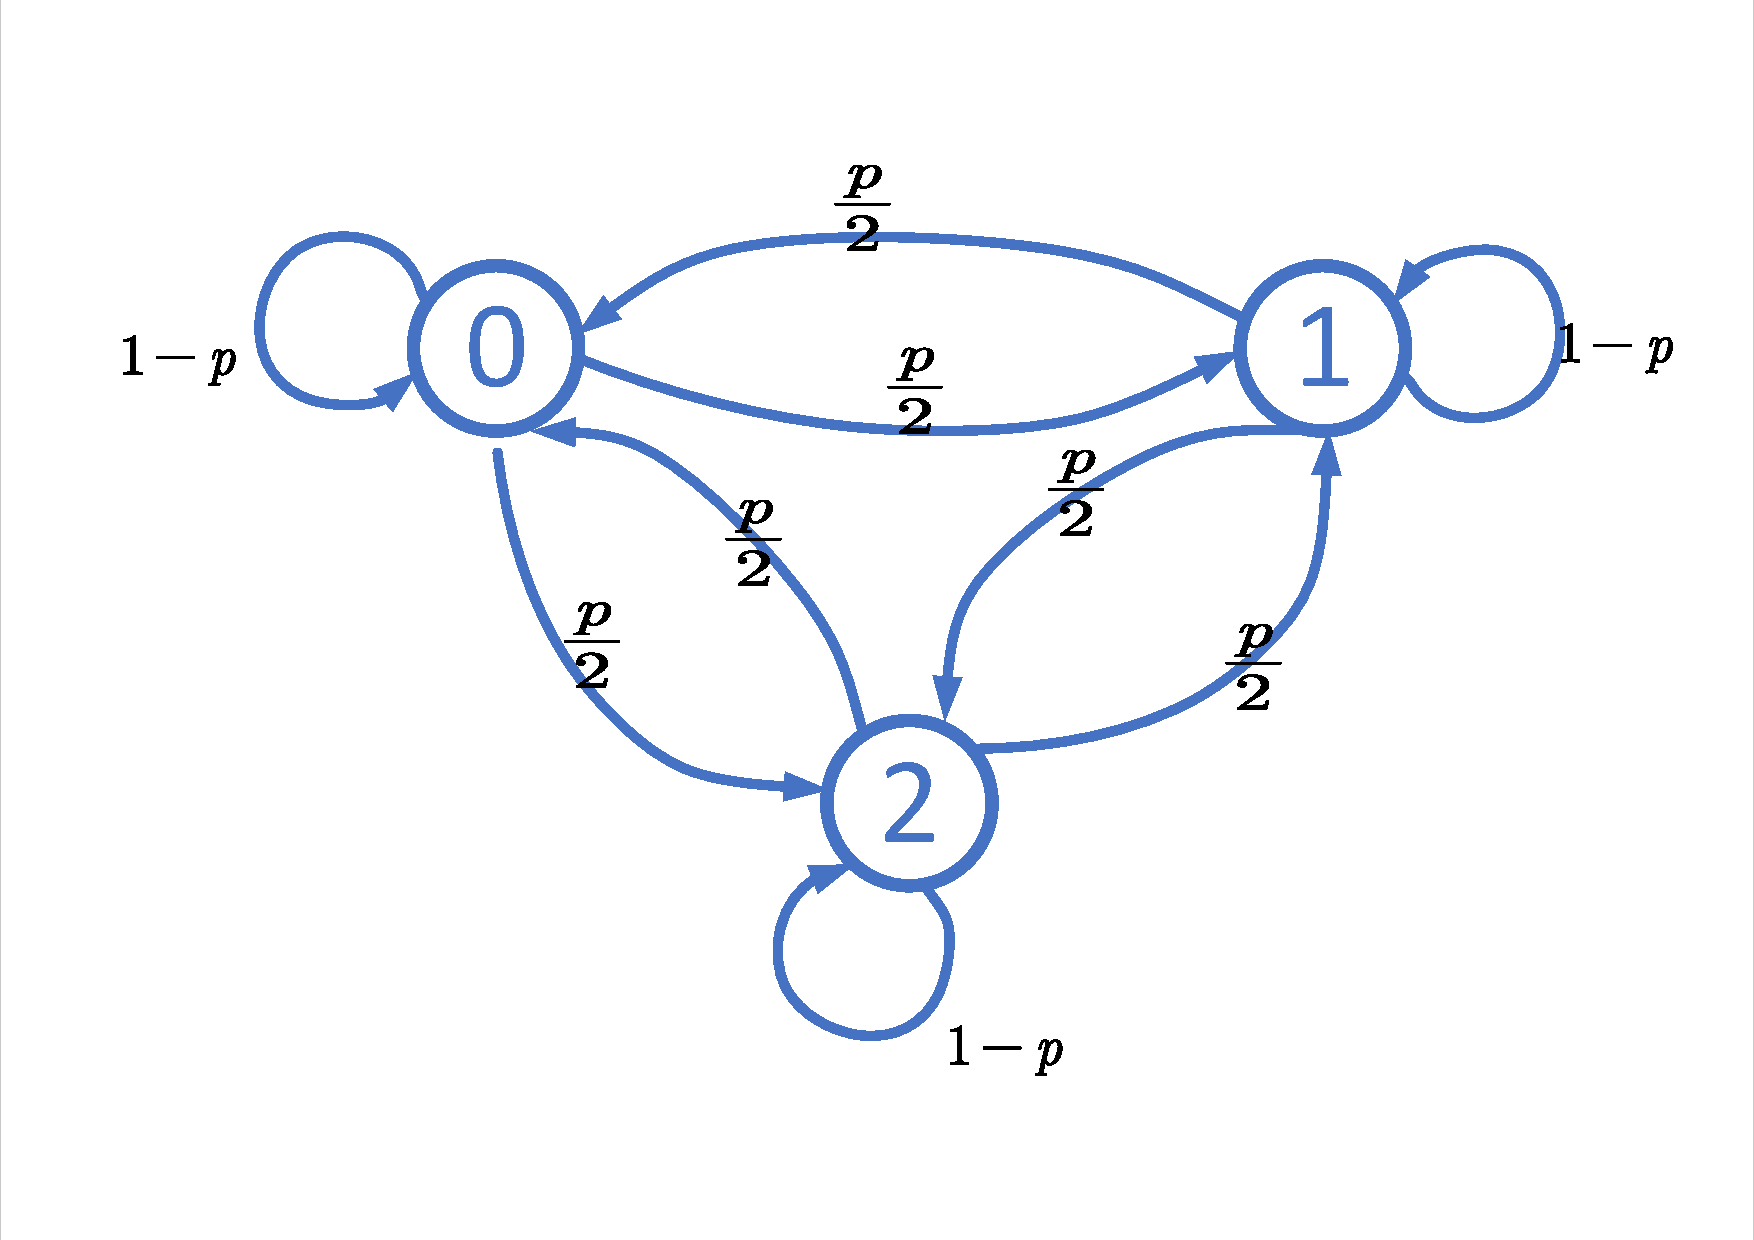
\includegraphics[width=0.45\textwidth]{figure/fig4.pdf}
    \end{figure}
    \begin{enumerate}
        \item 求信源的平稳分布;
        \vspace*{0.3cm}
        \item 求信源的符号熵;
        \vspace*{0.3cm}
        \item 当$p$为何值时,信源的符号熵达到最大值?
    \end{enumerate}
\end{enumerate}
\subsection*{五、信源编码:香农编码、哈夫曼编码、平均码长、信息传输率、编码效率}
\begin{enumerate}
    \item 信源空间为
    $$
    \begin{bmatrix}
        X\\
        P(X)
    \end{bmatrix} = \begin{bmatrix}
        x_1 & x_2 & x_3 & x_4 & x_5 & x_6 & x_7\\
        0.2 & 0.19 & 0.18 & 0.17 & 0.15 & 0.1 & 0.01\\
    \end{bmatrix}
    $$
    试分别构造二元香农码何二元霍夫曼码,写出编码过程并计算其平均码长、编码后的信息传输率何编码效率。
    \vspace*{0.8cm}
    \item 信源符号$X$有六钟字母,概率为0.32,0.22,0.18,0.16,0.08,0.04。试分别构造二元香农码和
    二元霍夫曼码,写出编码过程并计算其平均码长、编译后的信息传输率和编码效率。

\end{enumerate}
\subsection*{六、信道编码:信道容量、最佳入口分布}
\begin{enumerate}
    \item 在干扰离散对称信道上传输符号~1~和~0,已知$P(0)=\frac{1}{4}$, $P(1)=\frac{3}{4}$,试求:
    \begin{figure}[H]
        \centering
        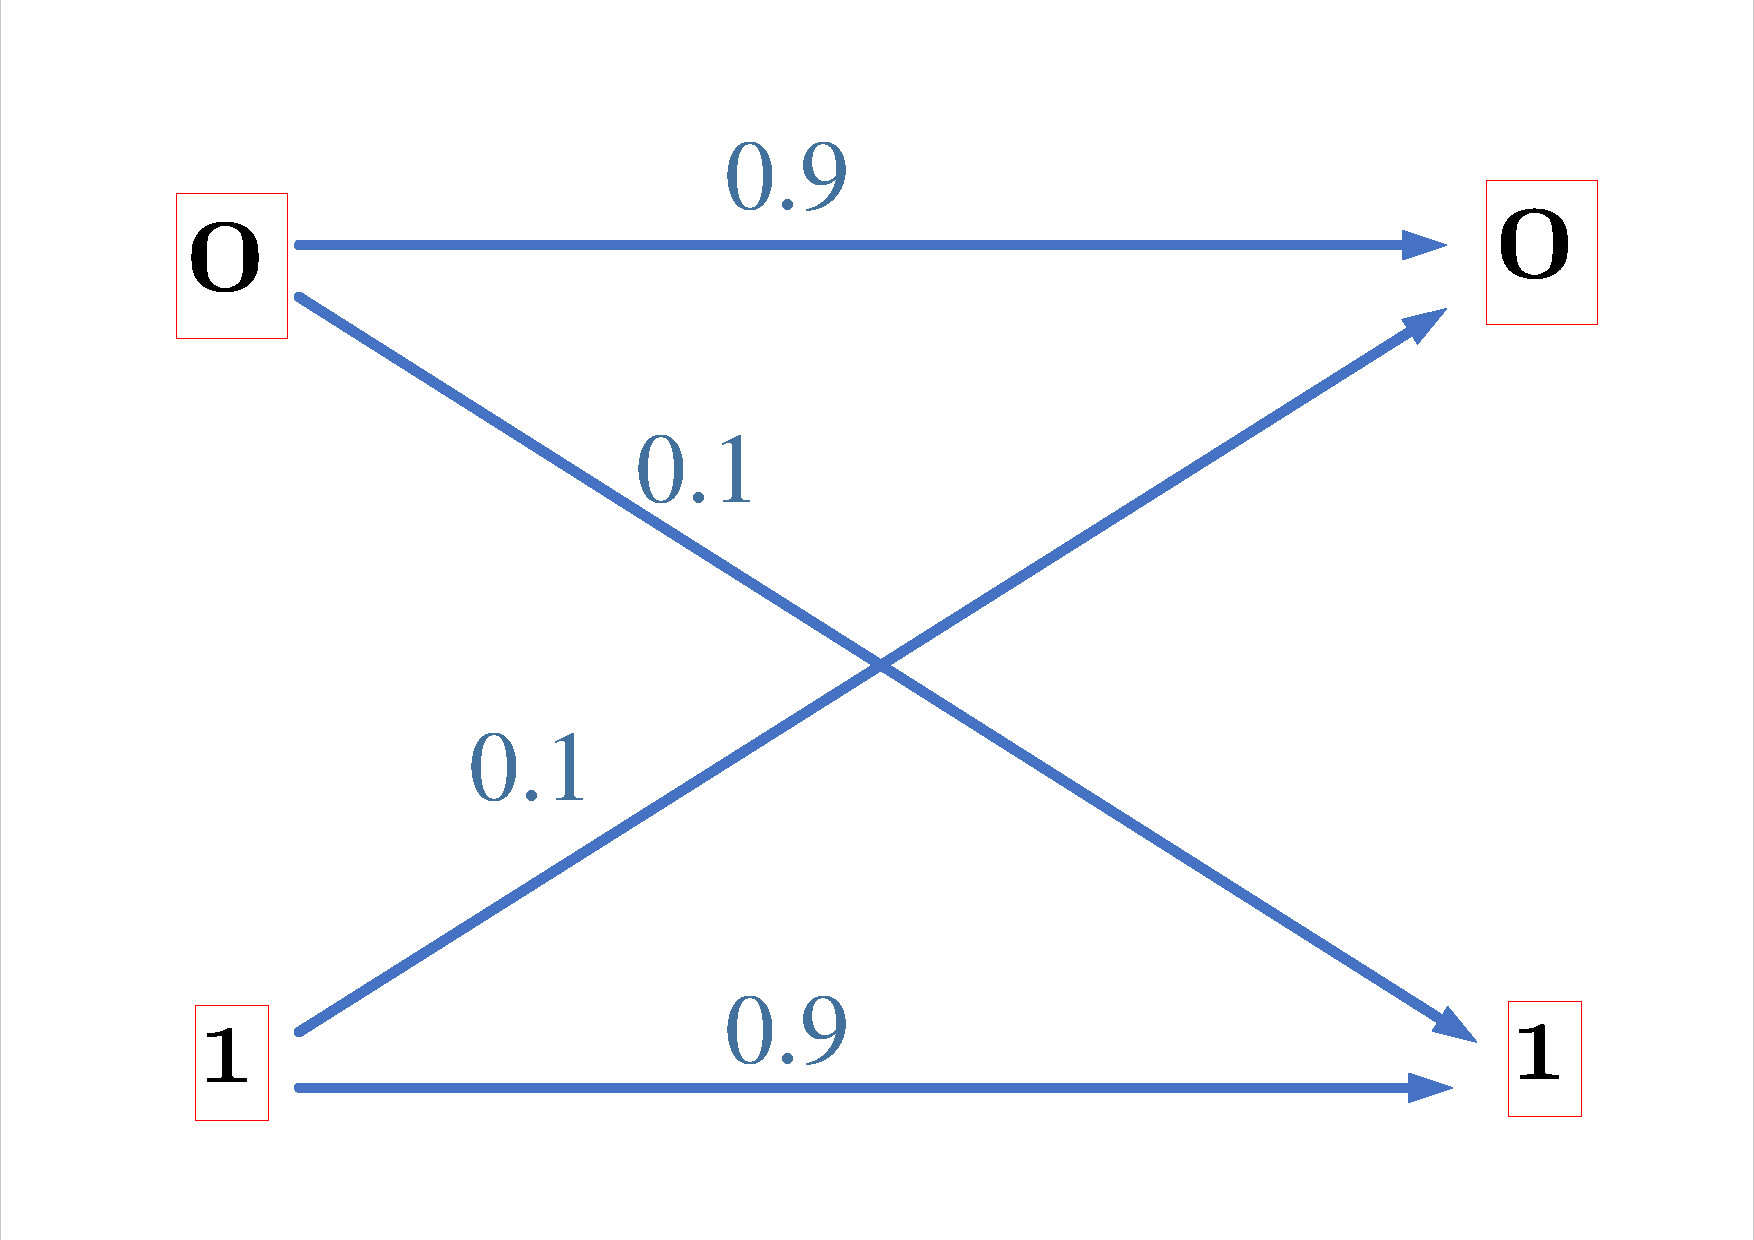
\includegraphics[width=0.45\textwidth]{figure/fig5.pdf}
    \end{figure}
    \begin{enumerate}
        \item 该信道的转移概率矩阵~$P$;
         \vspace*{0.3cm}
        \item 信道疑义度~$H(X|Y)$;
         \vspace*{0.3cm}
        \item 该信道的信道容量以及其输入概率分布。
    \end{enumerate}
    \vspace*{0.8cm}
    \item 信源发送端有~2~种符号$x_i(i=1,2)$, $p(x_1)=a$;接收端有~3~种符号$y_j(j=1,2,3)$,
    其概率矩阵为$P=\begin{bmatrix}
        1/2 & 1/2 & 0\\
        1/2 & 1/4 & 1/4
    \end{bmatrix}$。
    \begin{enumerate}
        \item 计算接收端的平均不确定度~$H(Y)$~;
        \vspace*{0.3cm}
        \item 计算由于噪声产生的不确定度~$H(Y|X)$~;
        \vspace*{0.3cm}
        \item 计算信道容量以及最佳入口分布。
    \end{enumerate}
\end{enumerate}
\end{document}